% !TEX TS-program = pdflatex
% !TEX encoding = UTF-8 Unicode
\documentclass[border=0mm]{standalone}
% packages
\usepackage{tikz}
\usetikzlibrary{patterns}
\usepackage{amsmath,amssymb}
\usepackage{bm}
\usepackage{pgfplots}
\pgfplotsset{compat=1.15}
% start document
\begin{document}
% generated by ROOT (CERN)
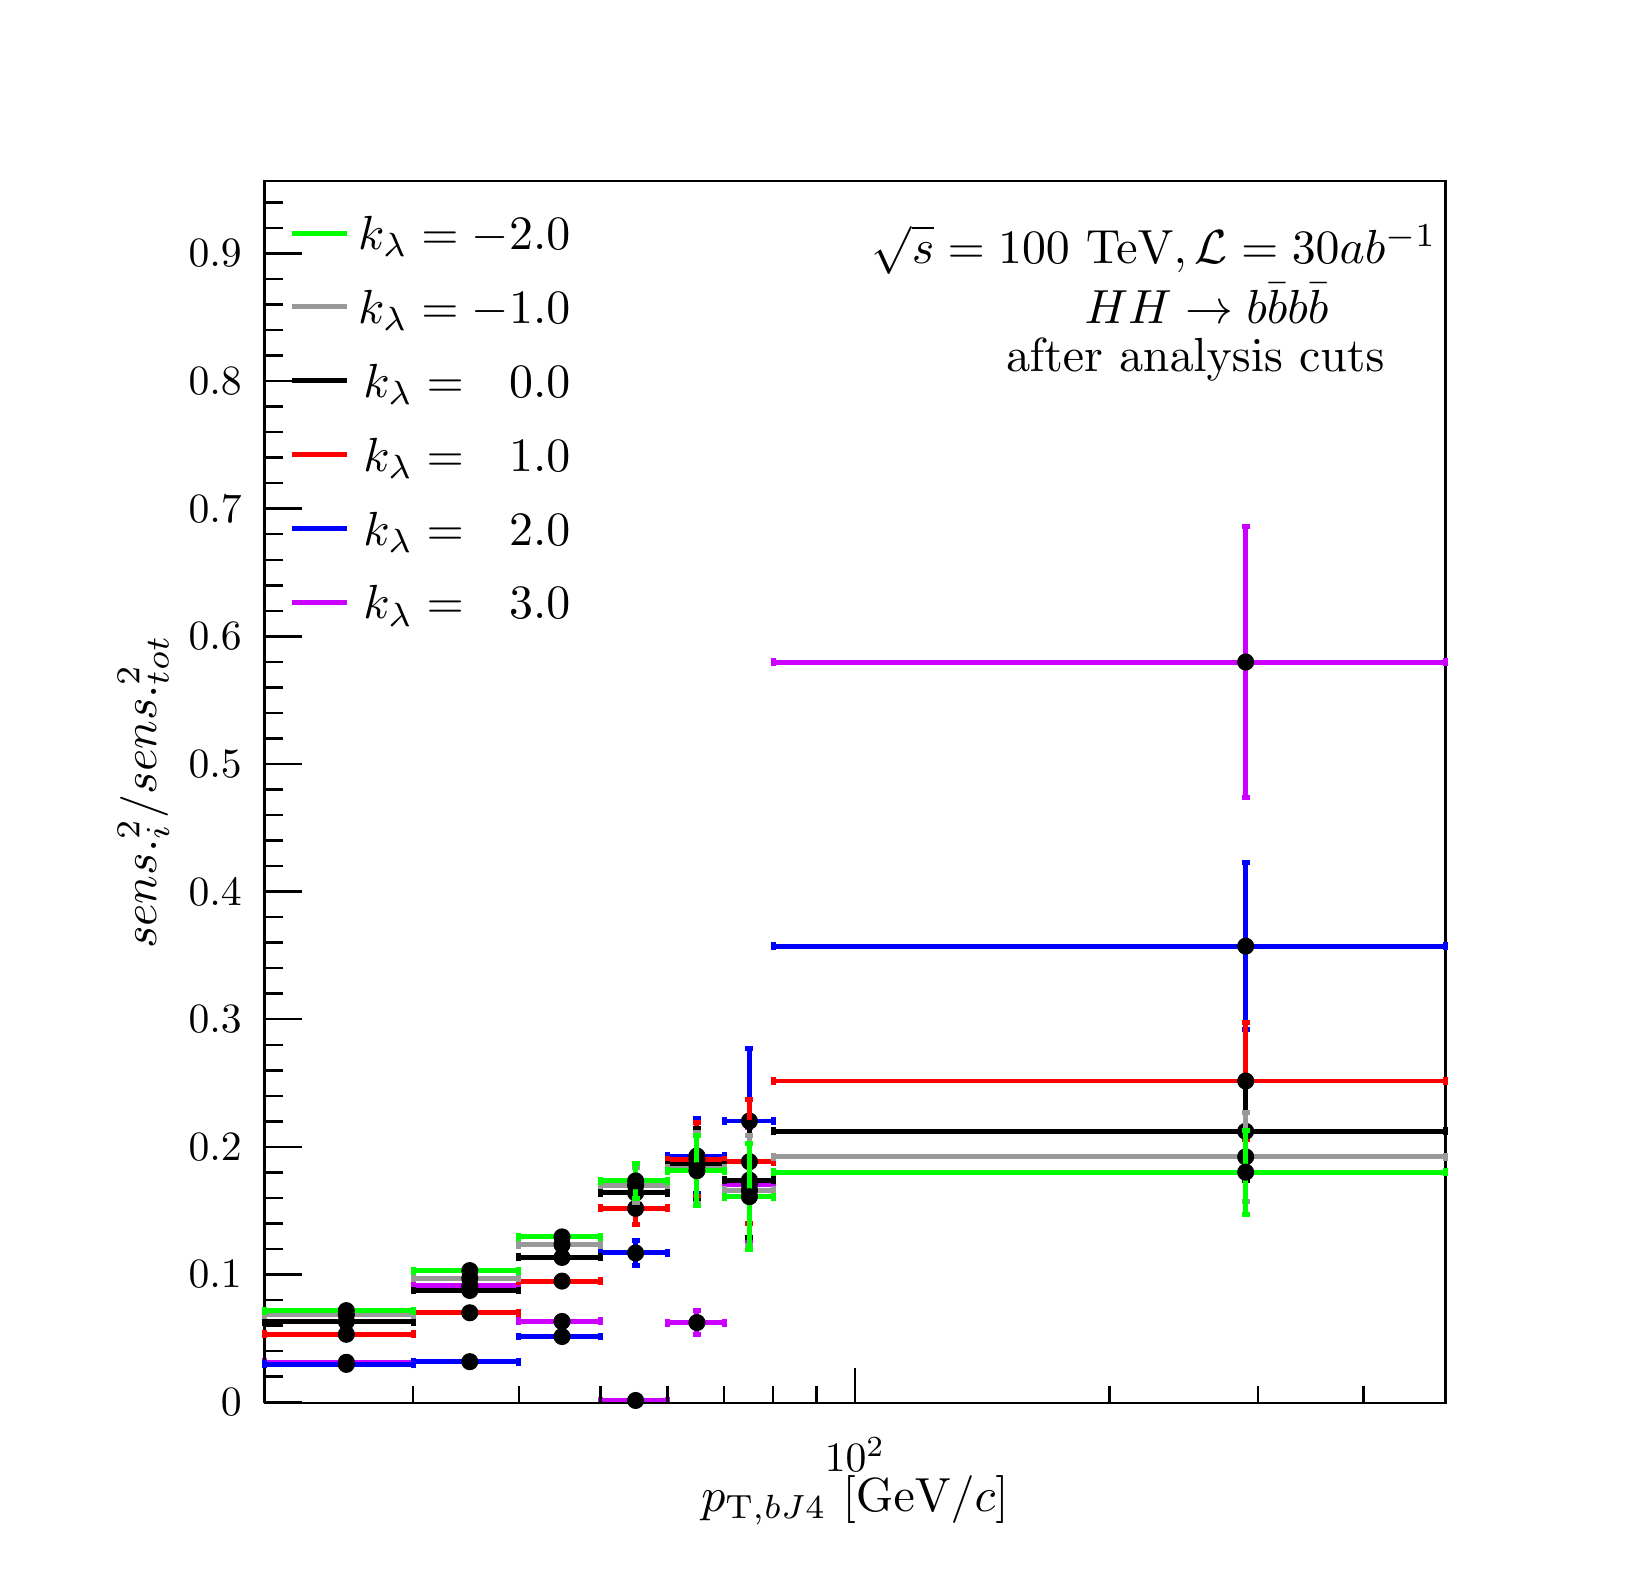
\begin{tikzpicture}
\pgfdeclareplotmark{cross} {
\pgfpathmoveto{\pgfpoint{-0.3\pgfplotmarksize}{\pgfplotmarksize}}
\pgfpathlineto{\pgfpoint{+0.3\pgfplotmarksize}{\pgfplotmarksize}}
\pgfpathlineto{\pgfpoint{+0.3\pgfplotmarksize}{0.3\pgfplotmarksize}}
\pgfpathlineto{\pgfpoint{+1\pgfplotmarksize}{0.3\pgfplotmarksize}}
\pgfpathlineto{\pgfpoint{+1\pgfplotmarksize}{-0.3\pgfplotmarksize}}
\pgfpathlineto{\pgfpoint{+0.3\pgfplotmarksize}{-0.3\pgfplotmarksize}}
\pgfpathlineto{\pgfpoint{+0.3\pgfplotmarksize}{-1.\pgfplotmarksize}}
\pgfpathlineto{\pgfpoint{-0.3\pgfplotmarksize}{-1.\pgfplotmarksize}}
\pgfpathlineto{\pgfpoint{-0.3\pgfplotmarksize}{-0.3\pgfplotmarksize}}
\pgfpathlineto{\pgfpoint{-1.\pgfplotmarksize}{-0.3\pgfplotmarksize}}
\pgfpathlineto{\pgfpoint{-1.\pgfplotmarksize}{0.3\pgfplotmarksize}}
\pgfpathlineto{\pgfpoint{-0.3\pgfplotmarksize}{0.3\pgfplotmarksize}}
\pgfpathclose
\pgfusepathqstroke
}
\pgfdeclareplotmark{cross*} {
\pgfpathmoveto{\pgfpoint{-0.3\pgfplotmarksize}{\pgfplotmarksize}}
\pgfpathlineto{\pgfpoint{+0.3\pgfplotmarksize}{\pgfplotmarksize}}
\pgfpathlineto{\pgfpoint{+0.3\pgfplotmarksize}{0.3\pgfplotmarksize}}
\pgfpathlineto{\pgfpoint{+1\pgfplotmarksize}{0.3\pgfplotmarksize}}
\pgfpathlineto{\pgfpoint{+1\pgfplotmarksize}{-0.3\pgfplotmarksize}}
\pgfpathlineto{\pgfpoint{+0.3\pgfplotmarksize}{-0.3\pgfplotmarksize}}
\pgfpathlineto{\pgfpoint{+0.3\pgfplotmarksize}{-1.\pgfplotmarksize}}
\pgfpathlineto{\pgfpoint{-0.3\pgfplotmarksize}{-1.\pgfplotmarksize}}
\pgfpathlineto{\pgfpoint{-0.3\pgfplotmarksize}{-0.3\pgfplotmarksize}}
\pgfpathlineto{\pgfpoint{-1.\pgfplotmarksize}{-0.3\pgfplotmarksize}}
\pgfpathlineto{\pgfpoint{-1.\pgfplotmarksize}{0.3\pgfplotmarksize}}
\pgfpathlineto{\pgfpoint{-0.3\pgfplotmarksize}{0.3\pgfplotmarksize}}
\pgfpathclose
\pgfusepathqfillstroke
}
\pgfdeclareplotmark{newstar} {
\pgfpathmoveto{\pgfqpoint{0pt}{\pgfplotmarksize}}
\pgfpathlineto{\pgfqpointpolar{44}{0.5\pgfplotmarksize}}
\pgfpathlineto{\pgfqpointpolar{18}{\pgfplotmarksize}}
\pgfpathlineto{\pgfqpointpolar{-20}{0.5\pgfplotmarksize}}
\pgfpathlineto{\pgfqpointpolar{-54}{\pgfplotmarksize}}
\pgfpathlineto{\pgfqpointpolar{-90}{0.5\pgfplotmarksize}}
\pgfpathlineto{\pgfqpointpolar{234}{\pgfplotmarksize}}
\pgfpathlineto{\pgfqpointpolar{198}{0.5\pgfplotmarksize}}
\pgfpathlineto{\pgfqpointpolar{162}{\pgfplotmarksize}}
\pgfpathlineto{\pgfqpointpolar{134}{0.5\pgfplotmarksize}}
\pgfpathclose
\pgfusepathqstroke
}
\pgfdeclareplotmark{newstar*} {
\pgfpathmoveto{\pgfqpoint{0pt}{\pgfplotmarksize}}
\pgfpathlineto{\pgfqpointpolar{44}{0.5\pgfplotmarksize}}
\pgfpathlineto{\pgfqpointpolar{18}{\pgfplotmarksize}}
\pgfpathlineto{\pgfqpointpolar{-20}{0.5\pgfplotmarksize}}
\pgfpathlineto{\pgfqpointpolar{-54}{\pgfplotmarksize}}
\pgfpathlineto{\pgfqpointpolar{-90}{0.5\pgfplotmarksize}}
\pgfpathlineto{\pgfqpointpolar{234}{\pgfplotmarksize}}
\pgfpathlineto{\pgfqpointpolar{198}{0.5\pgfplotmarksize}}
\pgfpathlineto{\pgfqpointpolar{162}{\pgfplotmarksize}}
\pgfpathlineto{\pgfqpointpolar{134}{0.5\pgfplotmarksize}}
\pgfpathclose
\pgfusepathqfillstroke
}
\definecolor{c}{rgb}{1,1,1};
\draw [color=c, fill=c] (0,0) rectangle (20,19.397);
\draw [color=c, fill=c] (3,1.9397) rectangle (18,17.4573);
\definecolor{c}{rgb}{0,0,0};
\draw [c,line width=0.9] (3,1.9397) -- (3,17.4573) -- (18,17.4573) -- (18,1.9397) -- (3,1.9397);
\definecolor{c}{rgb}{1,1,1};
\draw [color=c, fill=c] (3,1.9397) rectangle (18,17.4573);
\definecolor{c}{rgb}{0,0,0};
\draw [c,line width=0.9] (3,1.9397) -- (3,17.4573) -- (18,17.4573) -- (18,1.9397) -- (3,1.9397);
\definecolor{c}{rgb}{0.8,0,1};
\draw [c,line width=1.8] (3,2.4543) -- (3.93935,2.4543);
\draw [c,line width=1.8] (4.14035,2.4543) -- (4.88947,2.4543);
\draw [c,line width=1.8] (3,2.40405) -- (3,2.50455);
\draw [c,line width=1.8] (4.88947,2.40405) -- (4.88947,2.50455);
\definecolor{c}{rgb}{0,0,0};
\foreach \P in {(4.03985,2.4543)}{\draw[mark options={color=c,fill=c},mark size=2.882883pt,mark=*] plot coordinates {\P};}
\definecolor{c}{rgb}{0.8,0,1};
\draw [c,line width=1.8] (4.88947,3.42661) -- (5.50731,3.42661);
\draw [c,line width=1.8] (5.70832,3.42661) -- (6.23007,3.42661);
\draw [c,line width=1.8] (4.88947,3.37636) -- (4.88947,3.47686);
\draw [c,line width=1.8] (6.23007,3.37636) -- (6.23007,3.47686);
\definecolor{c}{rgb}{0,0,0};
\foreach \P in {(5.60782,3.42661)}{\draw[mark options={color=c,fill=c},mark size=2.882883pt,mark=*] plot coordinates {\P};}
\definecolor{c}{rgb}{0.8,0,1};
\draw [c,line width=1.8] (6.23007,2.97308) -- (6.67844,2.97308);
\draw [c,line width=1.8] (6.87945,2.97308) -- (7.26993,2.97308);
\draw [c,line width=1.8] (6.23007,2.92283) -- (6.23007,3.02333);
\draw [c,line width=1.8] (7.26993,2.92283) -- (7.26993,3.02333);
\definecolor{c}{rgb}{0,0,0};
\foreach \P in {(6.77894,2.97308)}{\draw[mark options={color=c,fill=c},mark size=2.882883pt,mark=*] plot coordinates {\P};}
\definecolor{c}{rgb}{0.8,0,1};
\draw [c,line width=1.8] (7.26993,1.96948) -- (7.61357,1.96948);
\draw [c,line width=1.8] (7.81458,1.96948) -- (8.11955,1.96948);
\draw [c,line width=1.8] (7.26993,1.91923) -- (7.26993,2.01973);
\draw [c,line width=1.8] (8.11955,1.91923) -- (8.11955,2.01973);
\definecolor{c}{rgb}{0,0,0};
\foreach \P in {(7.71407,1.96948)}{\draw[mark options={color=c,fill=c},mark size=2.882883pt,mark=*] plot coordinates {\P};}
\definecolor{c}{rgb}{0.8,0,1};
\draw [c,line width=1.8] (8.49255,2.80455) -- (8.49255,2.85814);
\draw [c,line width=1.8] (8.49255,3.05914) -- (8.49255,3.11273);
\draw [c,line width=1.8] (8.11955,2.95864) -- (8.39204,2.95864);
\draw [c,line width=1.8] (8.59305,2.95864) -- (8.83789,2.95864);
\draw [c,line width=1.8] (8.4423,2.80455) -- (8.5428,2.80455);
\draw [c,line width=1.8] (8.4423,3.11273) -- (8.5428,3.11273);
\draw [c,line width=1.8] (8.11955,2.90839) -- (8.11955,3.00889);
\draw [c,line width=1.8] (8.83789,2.90839) -- (8.83789,3.00889);
\definecolor{c}{rgb}{0,0,0};
\foreach \P in {(8.49255,2.95864)}{\draw[mark options={color=c,fill=c},mark size=2.882883pt,mark=*] plot coordinates {\P};}
\definecolor{c}{rgb}{0.8,0,1};
\draw [c,line width=1.8] (9.1594,4.00223) -- (9.1594,4.61667);
\draw [c,line width=1.8] (9.1594,4.81767) -- (9.1594,5.43212);
\draw [c,line width=1.8] (8.83789,4.71717) -- (9.0589,4.71717);
\draw [c,line width=1.8] (9.2599,4.71717) -- (9.46015,4.71717);
\draw [c,line width=1.8] (9.10915,4.00223) -- (9.20965,4.00223);
\draw [c,line width=1.8] (9.10915,5.43212) -- (9.20965,5.43212);
\draw [c,line width=1.8] (8.83789,4.66692) -- (8.83789,4.76742);
\draw [c,line width=1.8] (9.46015,4.66692) -- (9.46015,4.76742);
\definecolor{c}{rgb}{0,0,0};
\foreach \P in {(9.1594,4.71717)}{\draw[mark options={color=c,fill=c},mark size=2.882883pt,mark=*] plot coordinates {\P};}
\definecolor{c}{rgb}{0.8,0,1};
\draw [c,line width=1.8] (15.4616,9.63155) -- (15.4616,11.2471);
\draw [c,line width=1.8] (15.4616,11.4482) -- (15.4616,13.0637);
\draw [c,line width=1.8] (9.46015,11.3476) -- (15.3611,11.3476);
\draw [c,line width=1.8] (15.5621,11.3476) -- (18,11.3476);
\draw [c,line width=1.8] (15.4113,9.63155) -- (15.5118,9.63155);
\draw [c,line width=1.8] (15.4113,13.0637) -- (15.5118,13.0637);
\draw [c,line width=1.8] (9.46015,11.2974) -- (9.46015,11.3979);
\draw [c,line width=1.8] (18,11.2974) -- (18,11.3979);
\definecolor{c}{rgb}{0,0,0};
\foreach \P in {(15.4616,11.3476)}{\draw[mark options={color=c,fill=c},mark size=2.882883pt,mark=*] plot coordinates {\P};}
\draw [c,line width=0.9] (3,1.9397) -- (18,1.9397);
\draw [c,line width=0.9] (4.88946,2.15791) -- (4.88946,1.9397);
\draw [c,line width=0.9] (6.23007,2.15791) -- (6.23007,1.9397);
\draw [c,line width=0.9] (7.26992,2.15791) -- (7.26992,1.9397);
\draw [c,line width=0.9] (8.11954,2.15791) -- (8.11954,1.9397);
\draw [c,line width=0.9] (8.83788,2.15791) -- (8.83788,1.9397);
\draw [c,line width=0.9] (9.46014,2.15791) -- (9.46014,1.9397);
\draw [c,line width=0.9] (10.009,2.15791) -- (10.009,1.9397);
\draw [c,line width=0.9] (10.5,2.37613) -- (10.5,1.9397);
\draw [anchor=base] (10.5,1.06199) node[scale=1.50669, color=c, rotate=0]{$10^{2}$};
\draw [c,line width=0.9] (13.7301,2.15791) -- (13.7301,1.9397);
\draw [c,line width=0.9] (15.6195,2.15791) -- (15.6195,1.9397);
\draw [c,line width=0.9] (16.9601,2.15791) -- (16.9601,1.9397);
\draw (10.5,0.698292) node[scale=1.7299, color=c, rotate=0]{$p_{\text{T}, bJ4} ~[\text{GeV}/c]$};
\draw [c,line width=0.9] (3,1.9397) -- (3,17.4573);
\draw [c,line width=0.9] (3.48,1.94821) -- (3,1.94821);
\draw [c,line width=0.9] (3.24,2.2724) -- (3,2.2724);
\draw [c,line width=0.9] (3.24,2.59659) -- (3,2.59659);
\draw [c,line width=0.9] (3.24,2.92078) -- (3,2.92078);
\draw [c,line width=0.9] (3.24,3.24497) -- (3,3.24497);
\draw [c,line width=0.9] (3.48,3.56916) -- (3,3.56916);
\draw [c,line width=0.9] (3.24,3.89335) -- (3,3.89335);
\draw [c,line width=0.9] (3.24,4.21753) -- (3,4.21753);
\draw [c,line width=0.9] (3.24,4.54172) -- (3,4.54172);
\draw [c,line width=0.9] (3.24,4.86591) -- (3,4.86591);
\draw [c,line width=0.9] (3.48,5.1901) -- (3,5.1901);
\draw [c,line width=0.9] (3.24,5.51429) -- (3,5.51429);
\draw [c,line width=0.9] (3.24,5.83848) -- (3,5.83848);
\draw [c,line width=0.9] (3.24,6.16267) -- (3,6.16267);
\draw [c,line width=0.9] (3.24,6.48686) -- (3,6.48686);
\draw [c,line width=0.9] (3.48,6.81105) -- (3,6.81105);
\draw [c,line width=0.9] (3.24,7.13524) -- (3,7.13524);
\draw [c,line width=0.9] (3.24,7.45943) -- (3,7.45943);
\draw [c,line width=0.9] (3.24,7.78362) -- (3,7.78362);
\draw [c,line width=0.9] (3.24,8.10781) -- (3,8.10781);
\draw [c,line width=0.9] (3.48,8.432) -- (3,8.432);
\draw [c,line width=0.9] (3.24,8.75619) -- (3,8.75619);
\draw [c,line width=0.9] (3.24,9.08038) -- (3,9.08038);
\draw [c,line width=0.9] (3.24,9.40457) -- (3,9.40457);
\draw [c,line width=0.9] (3.24,9.72876) -- (3,9.72876);
\draw [c,line width=0.9] (3.48,10.0529) -- (3,10.0529);
\draw [c,line width=0.9] (3.24,10.3771) -- (3,10.3771);
\draw [c,line width=0.9] (3.24,10.7013) -- (3,10.7013);
\draw [c,line width=0.9] (3.24,11.0255) -- (3,11.0255);
\draw [c,line width=0.9] (3.24,11.3497) -- (3,11.3497);
\draw [c,line width=0.9] (3.48,11.6739) -- (3,11.6739);
\draw [c,line width=0.9] (3.24,11.9981) -- (3,11.9981);
\draw [c,line width=0.9] (3.24,12.3223) -- (3,12.3223);
\draw [c,line width=0.9] (3.24,12.6465) -- (3,12.6465);
\draw [c,line width=0.9] (3.24,12.9707) -- (3,12.9707);
\draw [c,line width=0.9] (3.48,13.2948) -- (3,13.2948);
\draw [c,line width=0.9] (3.24,13.619) -- (3,13.619);
\draw [c,line width=0.9] (3.24,13.9432) -- (3,13.9432);
\draw [c,line width=0.9] (3.24,14.2674) -- (3,14.2674);
\draw [c,line width=0.9] (3.24,14.5916) -- (3,14.5916);
\draw [c,line width=0.9] (3.48,14.9158) -- (3,14.9158);
\draw [c,line width=0.9] (3.24,15.24) -- (3,15.24);
\draw [c,line width=0.9] (3.24,15.5642) -- (3,15.5642);
\draw [c,line width=0.9] (3.24,15.8884) -- (3,15.8884);
\draw [c,line width=0.9] (3.24,16.2125) -- (3,16.2125);
\draw [c,line width=0.9] (3.48,16.5367) -- (3,16.5367);
\draw [c,line width=0.9] (3.48,1.94821) -- (3,1.94821);
\draw [c,line width=0.9] (3.48,16.5367) -- (3,16.5367);
\draw [c,line width=0.9] (3.24,16.8609) -- (3,16.8609);
\draw [c,line width=0.9] (3.24,17.1851) -- (3,17.1851);
\draw [anchor= east] (2.9,1.94821) node[scale=1.50669, color=c, rotate=0]{0};
\draw [anchor= east] (2.9,3.56916) node[scale=1.50669, color=c, rotate=0]{0.1};
\draw [anchor= east] (2.9,5.1901) node[scale=1.50669, color=c, rotate=0]{0.2};
\draw [anchor= east] (2.9,6.81105) node[scale=1.50669, color=c, rotate=0]{0.3};
\draw [anchor= east] (2.9,8.432) node[scale=1.50669, color=c, rotate=0]{0.4};
\draw [anchor= east] (2.9,10.0529) node[scale=1.50669, color=c, rotate=0]{0.5};
\draw [anchor= east] (2.9,11.6739) node[scale=1.50669, color=c, rotate=0]{0.6};
\draw [anchor= east] (2.9,13.2948) node[scale=1.50669, color=c, rotate=0]{0.7};
\draw [anchor= east] (2.9,14.9158) node[scale=1.50669, color=c, rotate=0]{0.8};
\draw [anchor= east] (2.9,16.5367) node[scale=1.50669, color=c, rotate=0]{0.9};
\draw (1.464,9.69849) node[scale=1.7299, color=c, rotate=90]{$sens._{i}^{2}/ sens._{tot}^{2}$};
\definecolor{c}{rgb}{0,0,1};
\draw [c,line width=1.8] (3,2.42786) -- (3.93935,2.42786);
\draw [c,line width=1.8] (4.14035,2.42786) -- (4.88947,2.42786);
\draw [c,line width=1.8] (3,2.37761) -- (3,2.47811);
\draw [c,line width=1.8] (4.88947,2.37761) -- (4.88947,2.47811);
\definecolor{c}{rgb}{0,0,0};
\foreach \P in {(4.03985,2.42786)}{\draw[mark options={color=c,fill=c},mark size=2.882883pt,mark=*] plot coordinates {\P};}
\definecolor{c}{rgb}{0,0,1};
\draw [c,line width=1.8] (4.88947,2.46229) -- (5.50731,2.46229);
\draw [c,line width=1.8] (5.70832,2.46229) -- (6.23007,2.46229);
\draw [c,line width=1.8] (4.88947,2.41204) -- (4.88947,2.51254);
\draw [c,line width=1.8] (6.23007,2.41204) -- (6.23007,2.51254);
\definecolor{c}{rgb}{0,0,0};
\foreach \P in {(5.60782,2.46229)}{\draw[mark options={color=c,fill=c},mark size=2.882883pt,mark=*] plot coordinates {\P};}
\definecolor{c}{rgb}{0,0,1};
\draw [c,line width=1.8] (6.23007,2.78175) -- (6.67844,2.78175);
\draw [c,line width=1.8] (6.87945,2.78175) -- (7.26993,2.78175);
\draw [c,line width=1.8] (6.23007,2.7315) -- (6.23007,2.832);
\draw [c,line width=1.8] (7.26993,2.7315) -- (7.26993,2.832);
\definecolor{c}{rgb}{0,0,0};
\foreach \P in {(6.77894,2.78175)}{\draw[mark options={color=c,fill=c},mark size=2.882883pt,mark=*] plot coordinates {\P};}
\definecolor{c}{rgb}{0,0,1};
\draw [c,line width=1.8] (7.71407,3.68952) -- (7.71407,3.74218);
\draw [c,line width=1.8] (7.71407,3.94318) -- (7.71407,3.99584);
\draw [c,line width=1.8] (7.26993,3.84268) -- (7.61357,3.84268);
\draw [c,line width=1.8] (7.81458,3.84268) -- (8.11955,3.84268);
\draw [c,line width=1.8] (7.66382,3.68952) -- (7.76432,3.68952);
\draw [c,line width=1.8] (7.66382,3.99584) -- (7.76432,3.99584);
\draw [c,line width=1.8] (7.26993,3.79243) -- (7.26993,3.89293);
\draw [c,line width=1.8] (8.11955,3.79243) -- (8.11955,3.89293);
\definecolor{c}{rgb}{0,0,0};
\foreach \P in {(7.71407,3.84268)}{\draw[mark options={color=c,fill=c},mark size=2.882883pt,mark=*] plot coordinates {\P};}
\definecolor{c}{rgb}{0,0,1};
\draw [c,line width=1.8] (8.49255,4.59749) -- (8.49255,4.97369);
\draw [c,line width=1.8] (8.49255,5.1747) -- (8.49255,5.5509);
\draw [c,line width=1.8] (8.11955,5.07419) -- (8.39204,5.07419);
\draw [c,line width=1.8] (8.59305,5.07419) -- (8.83789,5.07419);
\draw [c,line width=1.8] (8.4423,4.59749) -- (8.5428,4.59749);
\draw [c,line width=1.8] (8.4423,5.5509) -- (8.5428,5.5509);
\draw [c,line width=1.8] (8.11955,5.02394) -- (8.11955,5.12445);
\draw [c,line width=1.8] (8.83789,5.02394) -- (8.83789,5.12445);
\definecolor{c}{rgb}{0,0,0};
\foreach \P in {(8.49255,5.07419)}{\draw[mark options={color=c,fill=c},mark size=2.882883pt,mark=*] plot coordinates {\P};}
\definecolor{c}{rgb}{0,0,1};
\draw [c,line width=1.8] (9.1594,4.59682) -- (9.1594,5.41823);
\draw [c,line width=1.8] (9.1594,5.61923) -- (9.1594,6.44063);
\draw [c,line width=1.8] (8.83789,5.51873) -- (9.0589,5.51873);
\draw [c,line width=1.8] (9.2599,5.51873) -- (9.46015,5.51873);
\draw [c,line width=1.8] (9.10915,4.59682) -- (9.20965,4.59682);
\draw [c,line width=1.8] (9.10915,6.44063) -- (9.20965,6.44063);
\draw [c,line width=1.8] (8.83789,5.46848) -- (8.83789,5.56898);
\draw [c,line width=1.8] (9.46015,5.46848) -- (9.46015,5.56898);
\definecolor{c}{rgb}{0,0,0};
\foreach \P in {(9.1594,5.51873)}{\draw[mark options={color=c,fill=c},mark size=2.882883pt,mark=*] plot coordinates {\P};}
\definecolor{c}{rgb}{0,0,1};
\draw [c,line width=1.8] (15.4616,6.6821) -- (15.4616,7.63892);
\draw [c,line width=1.8] (15.4616,7.83993) -- (15.4616,8.79675);
\draw [c,line width=1.8] (9.46015,7.73943) -- (15.3611,7.73943);
\draw [c,line width=1.8] (15.5621,7.73943) -- (18,7.73943);
\draw [c,line width=1.8] (15.4113,6.6821) -- (15.5118,6.6821);
\draw [c,line width=1.8] (15.4113,8.79675) -- (15.5118,8.79675);
\draw [c,line width=1.8] (9.46015,7.68918) -- (9.46015,7.78968);
\draw [c,line width=1.8] (18,7.68918) -- (18,7.78968);
\definecolor{c}{rgb}{0,0,0};
\foreach \P in {(15.4616,7.73943)}{\draw[mark options={color=c,fill=c},mark size=2.882883pt,mark=*] plot coordinates {\P};}
\definecolor{c}{rgb}{1,0,0};
\draw [c,line width=1.8] (3,2.80995) -- (3.93935,2.80995);
\draw [c,line width=1.8] (4.14035,2.80995) -- (4.88947,2.80995);
\draw [c,line width=1.8] (3,2.7597) -- (3,2.8602);
\draw [c,line width=1.8] (4.88947,2.7597) -- (4.88947,2.8602);
\definecolor{c}{rgb}{0,0,0};
\foreach \P in {(4.03985,2.80995)}{\draw[mark options={color=c,fill=c},mark size=2.882883pt,mark=*] plot coordinates {\P};}
\definecolor{c}{rgb}{1,0,0};
\draw [c,line width=1.8] (4.88947,3.0834) -- (5.50731,3.0834);
\draw [c,line width=1.8] (5.70832,3.0834) -- (6.23007,3.0834);
\draw [c,line width=1.8] (4.88947,3.03315) -- (4.88947,3.13365);
\draw [c,line width=1.8] (6.23007,3.03315) -- (6.23007,3.13365);
\definecolor{c}{rgb}{0,0,0};
\foreach \P in {(5.60782,3.0834)}{\draw[mark options={color=c,fill=c},mark size=2.882883pt,mark=*] plot coordinates {\P};}
\definecolor{c}{rgb}{1,0,0};
\draw [c,line width=1.8] (6.23007,3.48575) -- (6.67844,3.48575);
\draw [c,line width=1.8] (6.87945,3.48575) -- (7.26993,3.48575);
\draw [c,line width=1.8] (6.23007,3.4355) -- (6.23007,3.53601);
\draw [c,line width=1.8] (7.26993,3.4355) -- (7.26993,3.53601);
\definecolor{c}{rgb}{0,0,0};
\foreach \P in {(6.77894,3.48575)}{\draw[mark options={color=c,fill=c},mark size=2.882883pt,mark=*] plot coordinates {\P};}
\definecolor{c}{rgb}{1,0,0};
\draw [c,line width=1.8] (7.71407,4.21019) -- (7.71407,4.30865);
\draw [c,line width=1.8] (7.71407,4.50965) -- (7.71407,4.6081);
\draw [c,line width=1.8] (7.26993,4.40915) -- (7.61357,4.40915);
\draw [c,line width=1.8] (7.81458,4.40915) -- (8.11955,4.40915);
\draw [c,line width=1.8] (7.66382,4.21019) -- (7.76432,4.21019);
\draw [c,line width=1.8] (7.66382,4.6081) -- (7.76432,4.6081);
\draw [c,line width=1.8] (7.26993,4.3589) -- (7.26993,4.4594);
\draw [c,line width=1.8] (8.11955,4.3589) -- (8.11955,4.4594);
\definecolor{c}{rgb}{0,0,0};
\foreach \P in {(7.71407,4.40915)}{\draw[mark options={color=c,fill=c},mark size=2.882883pt,mark=*] plot coordinates {\P};}
\definecolor{c}{rgb}{1,0,0};
\draw [c,line width=1.8] (8.49255,4.55969) -- (8.49255,4.92909);
\draw [c,line width=1.8] (8.49255,5.13009) -- (8.49255,5.4995);
\draw [c,line width=1.8] (8.11955,5.02959) -- (8.39204,5.02959);
\draw [c,line width=1.8] (8.59305,5.02959) -- (8.83789,5.02959);
\draw [c,line width=1.8] (8.4423,4.55969) -- (8.5428,4.55969);
\draw [c,line width=1.8] (8.4423,5.4995) -- (8.5428,5.4995);
\draw [c,line width=1.8] (8.11955,4.97934) -- (8.11955,5.07984);
\draw [c,line width=1.8] (8.83789,4.97934) -- (8.83789,5.07984);
\definecolor{c}{rgb}{0,0,0};
\foreach \P in {(8.49255,5.02959)}{\draw[mark options={color=c,fill=c},mark size=2.882883pt,mark=*] plot coordinates {\P};}
\definecolor{c}{rgb}{1,0,0};
\draw [c,line width=1.8] (9.1594,4.21379) -- (9.1594,4.90187);
\draw [c,line width=1.8] (9.1594,5.10288) -- (9.1594,5.79096);
\draw [c,line width=1.8] (8.83789,5.00238) -- (9.0589,5.00238);
\draw [c,line width=1.8] (9.2599,5.00238) -- (9.46015,5.00238);
\draw [c,line width=1.8] (9.10915,4.21379) -- (9.20965,4.21379);
\draw [c,line width=1.8] (9.10915,5.79096) -- (9.20965,5.79096);
\draw [c,line width=1.8] (8.83789,4.95212) -- (8.83789,5.05263);
\draw [c,line width=1.8] (9.46015,4.95212) -- (9.46015,5.05263);
\definecolor{c}{rgb}{0,0,0};
\foreach \P in {(9.1594,5.00238)}{\draw[mark options={color=c,fill=c},mark size=2.882883pt,mark=*] plot coordinates {\P};}
\definecolor{c}{rgb}{1,0,0};
\draw [c,line width=1.8] (15.4616,5.28208) -- (15.4616,5.9262);
\draw [c,line width=1.8] (15.4616,6.12721) -- (15.4616,6.77134);
\draw [c,line width=1.8] (9.46015,6.02671) -- (15.3611,6.02671);
\draw [c,line width=1.8] (15.5621,6.02671) -- (18,6.02671);
\draw [c,line width=1.8] (15.4113,5.28208) -- (15.5118,5.28208);
\draw [c,line width=1.8] (15.4113,6.77134) -- (15.5118,6.77134);
\draw [c,line width=1.8] (9.46015,5.97646) -- (9.46015,6.07696);
\draw [c,line width=1.8] (18,5.97646) -- (18,6.07696);
\definecolor{c}{rgb}{0,0,0};
\foreach \P in {(15.4616,6.02671)}{\draw[mark options={color=c,fill=c},mark size=2.882883pt,mark=*] plot coordinates {\P};}
\draw [c,line width=1.8] (3,2.97114) -- (3.93935,2.97114);
\draw [c,line width=1.8] (4.14035,2.97114) -- (4.88947,2.97114);
\draw [c,line width=1.8] (3,2.92089) -- (3,3.02139);
\draw [c,line width=1.8] (4.88947,2.92089) -- (4.88947,3.02139);
\foreach \P in {(4.03985,2.97114)}{\draw[mark options={color=c,fill=c},mark size=2.882883pt,mark=*] plot coordinates {\P};}
\draw [c,line width=1.8] (4.88947,3.36611) -- (5.50731,3.36611);
\draw [c,line width=1.8] (5.70832,3.36611) -- (6.23007,3.36611);
\draw [c,line width=1.8] (4.88947,3.31586) -- (4.88947,3.41636);
\draw [c,line width=1.8] (6.23007,3.31586) -- (6.23007,3.41636);
\foreach \P in {(5.60782,3.36611)}{\draw[mark options={color=c,fill=c},mark size=2.882883pt,mark=*] plot coordinates {\P};}
\draw [c,line width=1.8] (6.23007,3.78594) -- (6.67844,3.78594);
\draw [c,line width=1.8] (6.87945,3.78594) -- (7.26993,3.78594);
\draw [c,line width=1.8] (6.23007,3.73569) -- (6.23007,3.8362);
\draw [c,line width=1.8] (7.26993,3.73569) -- (7.26993,3.8362);
\foreach \P in {(6.77894,3.78594)}{\draw[mark options={color=c,fill=c},mark size=2.882883pt,mark=*] plot coordinates {\P};}
\draw [c,line width=1.8] (7.71407,4.39037) -- (7.71407,4.50467);
\draw [c,line width=1.8] (7.71407,4.70567) -- (7.71407,4.81997);
\draw [c,line width=1.8] (7.26993,4.60517) -- (7.61357,4.60517);
\draw [c,line width=1.8] (7.81458,4.60517) -- (8.11955,4.60517);
\draw [c,line width=1.8] (7.66382,4.39037) -- (7.76432,4.39037);
\draw [c,line width=1.8] (7.66382,4.81997) -- (7.76432,4.81997);
\draw [c,line width=1.8] (7.26993,4.55492) -- (7.26993,4.65542);
\draw [c,line width=1.8] (8.11955,4.55492) -- (8.11955,4.65542);
\foreach \P in {(7.71407,4.60517)}{\draw[mark options={color=c,fill=c},mark size=2.882883pt,mark=*] plot coordinates {\P};}
\draw [c,line width=1.8] (8.49255,4.50353) -- (8.49255,4.86284);
\draw [c,line width=1.8] (8.49255,5.06384) -- (8.49255,5.42314);
\draw [c,line width=1.8] (8.11955,4.96334) -- (8.39204,4.96334);
\draw [c,line width=1.8] (8.59305,4.96334) -- (8.83789,4.96334);
\draw [c,line width=1.8] (8.4423,4.50353) -- (8.5428,4.50353);
\draw [c,line width=1.8] (8.4423,5.42314) -- (8.5428,5.42314);
\draw [c,line width=1.8] (8.11955,4.91309) -- (8.11955,5.01359);
\draw [c,line width=1.8] (8.83789,4.91309) -- (8.83789,5.01359);
\foreach \P in {(8.49255,4.96334)}{\draw[mark options={color=c,fill=c},mark size=2.882883pt,mark=*] plot coordinates {\P};}
\draw [c,line width=1.8] (9.1594,4.03945) -- (9.1594,4.66685);
\draw [c,line width=1.8] (9.1594,4.86785) -- (9.1594,5.49525);
\draw [c,line width=1.8] (8.83789,4.76735) -- (9.0589,4.76735);
\draw [c,line width=1.8] (9.2599,4.76735) -- (9.46015,4.76735);
\draw [c,line width=1.8] (9.10915,4.03945) -- (9.20965,4.03945);
\draw [c,line width=1.8] (9.10915,5.49525) -- (9.20965,5.49525);
\draw [c,line width=1.8] (8.83789,4.7171) -- (8.83789,4.8176);
\draw [c,line width=1.8] (9.46015,4.7171) -- (9.46015,4.8176);
\foreach \P in {(9.1594,4.76735)}{\draw[mark options={color=c,fill=c},mark size=2.882883pt,mark=*] plot coordinates {\P};}
\draw [c,line width=1.8] (15.4616,4.75988) -- (15.4616,5.28738);
\draw [c,line width=1.8] (15.4616,5.48838) -- (15.4616,6.01587);
\draw [c,line width=1.8] (9.46015,5.38788) -- (15.3611,5.38788);
\draw [c,line width=1.8] (15.5621,5.38788) -- (18,5.38788);
\draw [c,line width=1.8] (15.4113,4.75988) -- (15.5118,4.75988);
\draw [c,line width=1.8] (15.4113,6.01587) -- (15.5118,6.01587);
\draw [c,line width=1.8] (9.46015,5.33763) -- (9.46015,5.43813);
\draw [c,line width=1.8] (18,5.33763) -- (18,5.43813);
\foreach \P in {(15.4616,5.38788)}{\draw[mark options={color=c,fill=c},mark size=2.882883pt,mark=*] plot coordinates {\P};}
\definecolor{c}{rgb}{0.6,0.6,0.6};
\draw [c,line width=1.8] (3,3.05726) -- (3.93935,3.05726);
\draw [c,line width=1.8] (4.14035,3.05726) -- (4.88947,3.05726);
\draw [c,line width=1.8] (3,3.00701) -- (3,3.10751);
\draw [c,line width=1.8] (4.88947,3.00701) -- (4.88947,3.10751);
\definecolor{c}{rgb}{0,0,0};
\foreach \P in {(4.03985,3.05726)}{\draw[mark options={color=c,fill=c},mark size=2.882883pt,mark=*] plot coordinates {\P};}
\definecolor{c}{rgb}{0.6,0.6,0.6};
\draw [c,line width=1.8] (4.88947,3.52135) -- (5.50731,3.52135);
\draw [c,line width=1.8] (5.70832,3.52135) -- (6.23007,3.52135);
\draw [c,line width=1.8] (4.88947,3.47109) -- (4.88947,3.5716);
\draw [c,line width=1.8] (6.23007,3.47109) -- (6.23007,3.5716);
\definecolor{c}{rgb}{0,0,0};
\foreach \P in {(5.60782,3.52135)}{\draw[mark options={color=c,fill=c},mark size=2.882883pt,mark=*] plot coordinates {\P};}
\definecolor{c}{rgb}{0.6,0.6,0.6};
\draw [c,line width=1.8] (6.23007,3.94698) -- (6.67844,3.94698);
\draw [c,line width=1.8] (6.87945,3.94698) -- (7.26993,3.94698);
\draw [c,line width=1.8] (6.23007,3.89673) -- (6.23007,3.99723);
\draw [c,line width=1.8] (7.26993,3.89673) -- (7.26993,3.99723);
\definecolor{c}{rgb}{0,0,0};
\foreach \P in {(6.77894,3.94698)}{\draw[mark options={color=c,fill=c},mark size=2.882883pt,mark=*] plot coordinates {\P};}
\definecolor{c}{rgb}{0.6,0.6,0.6};
\draw [c,line width=1.8] (7.71407,4.47864) -- (7.71407,4.6007);
\draw [c,line width=1.8] (7.71407,4.80171) -- (7.71407,4.92377);
\draw [c,line width=1.8] (7.26993,4.7012) -- (7.61357,4.7012);
\draw [c,line width=1.8] (7.81458,4.7012) -- (8.11955,4.7012);
\draw [c,line width=1.8] (7.66382,4.47864) -- (7.76432,4.47864);
\draw [c,line width=1.8] (7.66382,4.92377) -- (7.76432,4.92377);
\draw [c,line width=1.8] (7.26993,4.65095) -- (7.26993,4.75145);
\draw [c,line width=1.8] (8.11955,4.65095) -- (8.11955,4.75145);
\definecolor{c}{rgb}{0,0,0};
\foreach \P in {(7.71407,4.7012)}{\draw[mark options={color=c,fill=c},mark size=2.882883pt,mark=*] plot coordinates {\P};}
\definecolor{c}{rgb}{0.6,0.6,0.6};
\draw [c,line width=1.8] (8.49255,4.46539) -- (8.49255,4.81783);
\draw [c,line width=1.8] (8.49255,5.01883) -- (8.49255,5.37127);
\draw [c,line width=1.8] (8.11955,4.91833) -- (8.39204,4.91833);
\draw [c,line width=1.8] (8.59305,4.91833) -- (8.83789,4.91833);
\draw [c,line width=1.8] (8.4423,4.46539) -- (8.5428,4.46539);
\draw [c,line width=1.8] (8.4423,5.37127) -- (8.5428,5.37127);
\draw [c,line width=1.8] (8.11955,4.86808) -- (8.11955,4.96858);
\draw [c,line width=1.8] (8.83789,4.86808) -- (8.83789,4.96858);
\definecolor{c}{rgb}{0,0,0};
\foreach \P in {(8.49255,4.91833)}{\draw[mark options={color=c,fill=c},mark size=2.882883pt,mark=*] plot coordinates {\P};}
\definecolor{c}{rgb}{0.6,0.6,0.6};
\draw [c,line width=1.8] (9.1594,3.94372) -- (9.1594,4.5378);
\draw [c,line width=1.8] (9.1594,4.7388) -- (9.1594,5.33288);
\draw [c,line width=1.8] (8.83789,4.6383) -- (9.0589,4.6383);
\draw [c,line width=1.8] (9.2599,4.6383) -- (9.46015,4.6383);
\draw [c,line width=1.8] (9.10915,3.94372) -- (9.20965,3.94372);
\draw [c,line width=1.8] (9.10915,5.33288) -- (9.20965,5.33288);
\draw [c,line width=1.8] (8.83789,4.58805) -- (8.83789,4.68855);
\draw [c,line width=1.8] (9.46015,4.58805) -- (9.46015,4.68855);
\definecolor{c}{rgb}{0,0,0};
\foreach \P in {(9.1594,4.6383)}{\draw[mark options={color=c,fill=c},mark size=2.882883pt,mark=*] plot coordinates {\P};}
\definecolor{c}{rgb}{0.6,0.6,0.6};
\draw [c,line width=1.8] (15.4616,4.49474) -- (15.4616,4.96301);
\draw [c,line width=1.8] (15.4616,5.16402) -- (15.4616,5.63229);
\draw [c,line width=1.8] (9.46015,5.06351) -- (15.3611,5.06351);
\draw [c,line width=1.8] (15.5621,5.06351) -- (18,5.06351);
\draw [c,line width=1.8] (15.4113,4.49474) -- (15.5118,4.49474);
\draw [c,line width=1.8] (15.4113,5.63229) -- (15.5118,5.63229);
\draw [c,line width=1.8] (9.46015,5.01326) -- (9.46015,5.11376);
\draw [c,line width=1.8] (18,5.01326) -- (18,5.11376);
\definecolor{c}{rgb}{0,0,0};
\foreach \P in {(15.4616,5.06351)}{\draw[mark options={color=c,fill=c},mark size=2.882883pt,mark=*] plot coordinates {\P};}
\definecolor{c}{rgb}{0,1,0};
\draw [c,line width=1.8] (3,3.11046) -- (3.93935,3.11046);
\draw [c,line width=1.8] (4.14035,3.11046) -- (4.88947,3.11046);
\draw [c,line width=1.8] (3,3.06021) -- (3,3.16072);
\draw [c,line width=1.8] (4.88947,3.06021) -- (4.88947,3.16072);
\definecolor{c}{rgb}{0,0,0};
\foreach \P in {(4.03985,3.11046)}{\draw[mark options={color=c,fill=c},mark size=2.882883pt,mark=*] plot coordinates {\P};}
\definecolor{c}{rgb}{0,1,0};
\draw [c,line width=1.8] (4.88947,3.61865) -- (5.50731,3.61865);
\draw [c,line width=1.8] (5.70832,3.61865) -- (6.23007,3.61865);
\draw [c,line width=1.8] (4.88947,3.5684) -- (4.88947,3.6689);
\draw [c,line width=1.8] (6.23007,3.5684) -- (6.23007,3.6689);
\definecolor{c}{rgb}{0,0,0};
\foreach \P in {(5.60782,3.61865)}{\draw[mark options={color=c,fill=c},mark size=2.882883pt,mark=*] plot coordinates {\P};}
\definecolor{c}{rgb}{0,1,0};
\draw [c,line width=1.8] (6.23007,4.04669) -- (6.67844,4.04669);
\draw [c,line width=1.8] (6.87945,4.04669) -- (7.26993,4.04669);
\draw [c,line width=1.8] (6.23007,3.99643) -- (6.23007,4.09694);
\draw [c,line width=1.8] (7.26993,3.99643) -- (7.26993,4.09694);
\definecolor{c}{rgb}{0,0,0};
\foreach \P in {(6.77894,4.04669)}{\draw[mark options={color=c,fill=c},mark size=2.882883pt,mark=*] plot coordinates {\P};}
\definecolor{c}{rgb}{0,1,0};
\draw [c,line width=1.8] (7.71407,4.5305) -- (7.71407,4.65713);
\draw [c,line width=1.8] (7.71407,4.85813) -- (7.71407,4.98476);
\draw [c,line width=1.8] (7.26993,4.75763) -- (7.61357,4.75763);
\draw [c,line width=1.8] (7.81458,4.75763) -- (8.11955,4.75763);
\draw [c,line width=1.8] (7.66382,4.5305) -- (7.76432,4.5305);
\draw [c,line width=1.8] (7.66382,4.98476) -- (7.76432,4.98476);
\draw [c,line width=1.8] (7.26993,4.70738) -- (7.26993,4.80788);
\draw [c,line width=1.8] (8.11955,4.70738) -- (8.11955,4.80788);
\definecolor{c}{rgb}{0,0,0};
\foreach \P in {(7.71407,4.75763)}{\draw[mark options={color=c,fill=c},mark size=2.882883pt,mark=*] plot coordinates {\P};}
\definecolor{c}{rgb}{0,1,0};
\draw [c,line width=1.8] (8.49255,4.43911) -- (8.49255,4.78682);
\draw [c,line width=1.8] (8.49255,4.98782) -- (8.49255,5.33553);
\draw [c,line width=1.8] (8.11955,4.88732) -- (8.39204,4.88732);
\draw [c,line width=1.8] (8.59305,4.88732) -- (8.83789,4.88732);
\draw [c,line width=1.8] (8.4423,4.43911) -- (8.5428,4.43911);
\draw [c,line width=1.8] (8.4423,5.33553) -- (8.5428,5.33553);
\draw [c,line width=1.8] (8.11955,4.83707) -- (8.11955,4.93757);
\draw [c,line width=1.8] (8.83789,4.83707) -- (8.83789,4.93757);
\definecolor{c}{rgb}{0,0,0};
\foreach \P in {(8.49255,4.88732)}{\draw[mark options={color=c,fill=c},mark size=2.882883pt,mark=*] plot coordinates {\P};}
\definecolor{c}{rgb}{0,1,0};
\draw [c,line width=1.8] (9.1594,3.88371) -- (9.1594,4.4569);
\draw [c,line width=1.8] (9.1594,4.65791) -- (9.1594,5.2311);
\draw [c,line width=1.8] (8.83789,4.55741) -- (9.0589,4.55741);
\draw [c,line width=1.8] (9.2599,4.55741) -- (9.46015,4.55741);
\draw [c,line width=1.8] (9.10915,3.88371) -- (9.20965,3.88371);
\draw [c,line width=1.8] (9.10915,5.2311) -- (9.20965,5.2311);
\draw [c,line width=1.8] (8.83789,4.50716) -- (8.83789,4.60766);
\draw [c,line width=1.8] (9.46015,4.50716) -- (9.46015,4.60766);
\definecolor{c}{rgb}{0,0,0};
\foreach \P in {(9.1594,4.55741)}{\draw[mark options={color=c,fill=c},mark size=2.882883pt,mark=*] plot coordinates {\P};}
\definecolor{c}{rgb}{0,1,0};
\draw [c,line width=1.8] (15.4616,4.33555) -- (15.4616,4.76827);
\draw [c,line width=1.8] (15.4616,4.96928) -- (15.4616,5.40199);
\draw [c,line width=1.8] (9.46015,4.86877) -- (15.3611,4.86877);
\draw [c,line width=1.8] (15.5621,4.86877) -- (18,4.86877);
\draw [c,line width=1.8] (15.4113,4.33555) -- (15.5118,4.33555);
\draw [c,line width=1.8] (15.4113,5.40199) -- (15.5118,5.40199);
\draw [c,line width=1.8] (9.46015,4.81852) -- (9.46015,4.91902);
\draw [c,line width=1.8] (18,4.81852) -- (18,4.91902);
\definecolor{c}{rgb}{0,0,0};
\foreach \P in {(15.4616,4.86877)}{\draw[mark options={color=c,fill=c},mark size=2.882883pt,mark=*] plot coordinates {\P};}
\draw [anchor=base east] (7.1,16.5836) node[scale=1.7299, color=c, rotate=0]{$k_{\lambda} = -2.0$};
\definecolor{c}{rgb}{0,1,0};
\draw [c,line width=1.8] (3.35,16.7946) -- (4.05,16.7946);
\definecolor{c}{rgb}{0,0,0};
\draw [anchor=base east] (7.1,15.6461) node[scale=1.7299, color=c, rotate=0]{$k_{\lambda} = -1.0$};
\definecolor{c}{rgb}{0.6,0.6,0.6};
\draw [c,line width=1.8] (3.35,15.857) -- (4.05,15.857);
\definecolor{c}{rgb}{0,0,0};
\draw [anchor=base east] (7.1,14.7086) node[scale=1.7299, color=c, rotate=0]{$k_{\lambda} =~~0.0$};
\draw [c,line width=1.8] (3.35,14.9195) -- (4.05,14.9195);
\draw [anchor=base east] (7.1,13.7711) node[scale=1.7299, color=c, rotate=0]{$k_{\lambda} =~~1.0$};
\definecolor{c}{rgb}{1,0,0};
\draw [c,line width=1.8] (3.35,13.982) -- (4.05,13.982);
\definecolor{c}{rgb}{0,0,0};
\draw [anchor=base east] (7.1,12.8335) node[scale=1.7299, color=c, rotate=0]{$k_{\lambda} =~~2.0$};
\definecolor{c}{rgb}{0,0,1};
\draw [c,line width=1.8] (3.35,13.0445) -- (4.05,13.0445);
\definecolor{c}{rgb}{0,0,0};
\draw [anchor=base east] (7.1,11.896) node[scale=1.7299, color=c, rotate=0]{$k_{\lambda} =~~3.0$};
\definecolor{c}{rgb}{0.8,0,1};
\draw [c,line width=1.8] (3.35,12.107) -- (4.05,12.107);
\definecolor{c}{rgb}{0,0,0};
\draw [anchor= west] (10.5,16.5844) node[scale=1.7299, color=c, rotate=0]{$\sqrt{s} = 100 ~\text{TeV}, \mathcal{L} = 30 ab^{-1}$};
\draw [anchor= west] (13.2,15.9055) node[scale=1.7299, color=c, rotate=0]{$HH \rightarrow b\bar{b}b\bar{b}$};
\draw [anchor=base west] (12.2,15.0424) node[scale=1.7299, color=c, rotate=0]{after analysis cuts};
\end{tikzpicture}
% end document
\end{document}
